\subsection{Premessa e presentazione}
    \begin{figure}[H]
        \centering
        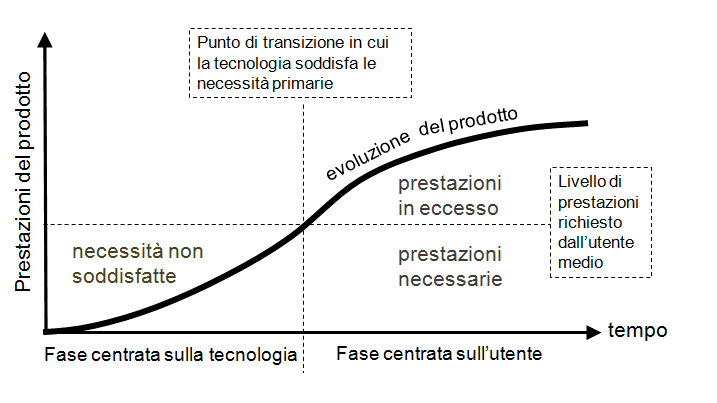
\includegraphics[scale=0.5]{assets/immagini varie/D.Norman grafico.png}
        \caption{\textbf{Grafico}: Evoluzione dei prodotti high-tech secondo D.Norman}\label{fig:Mockup_Homepage}
    \end{figure}

    \begin{flushleft}
        Con questo piccolo preambolo vogliamo richiamare l'attenzione sul diagramma di evoluzione dei prodotti software di D.Norman,
        il quale mostra il ciclo di vita che solitamente questo tipo di prodotto ha.
        All'inizio avremo un'app più incentrata sulle tecnologie implementate e/o da implementare per  "cercare " di
        raggiungere ciò che l'utente medio richiede dall'applicativo. Successivamente si otterrà il punto di pareggio in cui si soddisfano
        i bisogni dell'utente tipico, e ciò potrebbe essere considerato un buon punto di equilibrio del sistema.
        In fine, sempre ammesso che l'app sia sopravvissuta al mercato durante questo ciclo, ci può essere una fase finale con una condizione
        di iperfunzionalità, dove si cercherà via via di soddisfarre le esigenze di una platea di utenti più ampia.
        Nel caso della nostra applicazione Ratatouille23 descritta in questo documento, pensiamo di distribuire un prodotto nella sua 
        fase di equilibrio (vedere grafico) che certamente soddisfa le esigenze degli attori utilizzatori descritti nei punti successivi, 
        ma che allo stesso tempo può essere facilmente aggiornata e migliorata qualora dovessero aggiungersi nuovi target d'utenti o cambiare
        gli esistenti.
    \end{flushleft}
 